%!TEX root = Main.tex
\documentclass[Main]{subfiles}

\begin{document}
\section{PID} % (fold)
	\label{sec:pid}
This lesson covers path smoothing, and control using PID controllers.

\subsection{Path smoothing}
Path smoothing is an extension to the material from previous lesson, where the generation of paths was covered. 
In this section it is explored how these paths can be smoothed to better fit the motion model of, for example, a car. 
An example of this can be seen in \autoref{fig:path_smoothing}.
\begin{figure}[H]
	\centering
	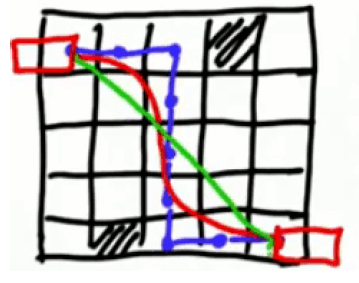
\includegraphics[scale=1]{./Figures/path_smoothing.png}
	\caption{Path smoothing}
	\label{fig:path_smoothing}
\end{figure}\noindent
In this figure, the red path is a smoothed version of the blue path. 
This path fits the motion model of a car much better than the blue or the green path, since a car cannot do perfect 45 or 90-degree turns.

The proposed smoothing algorithm works as follows:
\begin{itemize}
	\item Given a original path, $\overrightarrow{p}$, which consists of multiple x,y coordinates
	\begin{equation}
		p_i = [x_i,y_i]
	\end{equation}
	\item Create a copy of the original path, which will hold the smoothed points
	\begin{equation}
		\overrightarrow{s} = \overrightarrow{p}
	\end{equation}
	\item Minimize the distance between the original path, and the smoothed path
	\begin{equation}
		\min_{s_i}(p_i-s_i)^2
	\end{equation}
	\item While also minimizing the distance between the consecutive points in the smoothed path
	\begin{equation}
		\min_{s_i}(s_i-s_{i+1})^2
	\end{equation}
	\item Using gradient decent
	\begin{equation}
		s_i = s_i + \alpha \cdot (p_i + s_i) + \beta \cdot (s_{i+1} + s_{i-1} - 2 \cdot s_i)
	\end{equation}
	\item Until the accumulated change is below a certain threshold
\end{itemize}
% subsection path smoothing (end)

\subsection{PID controllers}
In this section the PID controller is covered and Cross Track Error is introduced.
\begin{figure}[H]
	\centering
	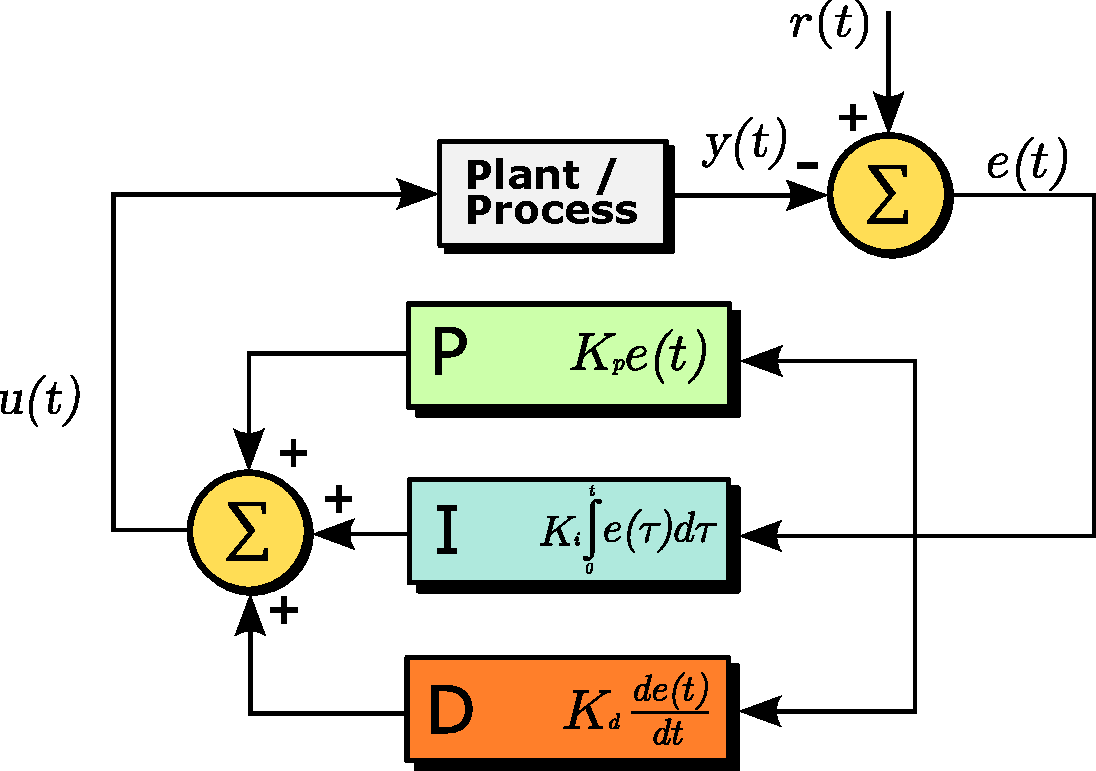
\includegraphics[scale=0.5]{PIDblock}
	\caption{PID controller block diagram}
	\label{fig:pid_controller}
\end{figure}\noindent
A PID controller, is a controller that produces a control signal, u(t)  that minimizes a certain error, e(t) , by using P(Proportionality), I(integration) and D(differentiation). 
In the examples in this course, the error is the Cross Track Error (CTE), which is the difference between the robots current position, and the expected position on the robots current path, calculated from the robots center of mass.

The different parts of a PID controlled assess different problems, and as such some parts, might be left out.

In a simple P controller, the error will only be scaled. 
Therefore a P controller will always overshoot, and be marginally stable.
\begin{equation}
	u = \tau_p \cdot CTE
\end{equation}
By introducing a differentiator, the controller avoids overshoot.
\begin{equation}
	u = \tau_p \cdot CTE - \tau_d \cdot \frac{d}{dt} CTE
\end{equation}
And by introducing an integrator, bias can be avoided.
\begin{equation}
	u = \tau_p \cdot CTE - \tau_d \cdot \frac{d}{dt} CTE - \tau_i \cdot \int CTE dt
\end{equation}
% subsection pid controllers (end)

\subsection{Twiddle/Coordinate Descent}

\fxnote{Måge: skriv ind på en god måde :)}
Coordinate descent is a proposed method for finding the parameters $\tau_p$, $\tau_d$ and $\tau_i$ for the PID controller, where the parameters iteratively are corrected towards a better value.

The algorithm for coordinated decent is as follows:
\begin{enumerate}
\item Build a parameter vector, $\mathbf{p} = [0,0,0]$
\item Build a vector of potential changes, $\mathbf{dp} = [1,1,1]$
\item Add the potential change to the parameter at index i, $\mathbf{p}_i = \mathbf{p}_i + \mathbf{dp}_i$
\item Calculate the CTE
\item Check if the calculated CTE is smaller than the previous best, $CTE_{calc} < CTE_{best}$
\item if true
\begin{enumerate}
	\item Set the calculated CTE to the best CTE, $CTE_{best} = CTE_{calc}$
	\item Update the potential to a larger value, $\mathbf{dp}_i = \mathbf{dp}_i \cdot 1.1$
	\item Go to step 3
\end{enumerate}
\item if false
\begin{enumerate}
	\item Subtract the potential change from the original parameter at index i, $\mathbf{p}_i = \mathbf{p}_i - 2 \cdot \mathbf{dp}_i$
	\item Calculate the CTE
	\item  Check if the calculated CTE is smaller than the previous best, $CTE_{calc} < CTE_{best}$
	\item if true
	\begin{enumerate}
		\item Set the calculated CTE to the best CTE, $CTE_{best} = CTE_{calc}$
		\item Update the potential to a larger value, $\mathbf{dp}_i = \mathbf{dp}_i \cdot 1.1$
	\end{enumerate}
	\item if false
	\begin{enumerate}
		\item Update the potential to a smaller value, $\mathbf{dp}_i = \mathbf{dp}_i \cdot 0.9$
	\end{enumerate}
	\item Go to step 3
\end{enumerate}
\end{enumerate} \fxnote{skal det være pseudokode istedet for?}
This is done while sum of potential changes is larger than a given threshold, and repeats for all the parameters.
As can be seen, the algorithm basically start by adding a change to one of the parameter.
If this gives a better CTE, it makes the change for the next iteration bigger.
If it is worse, it tries to subtract the change instead.
It then checks the CTE again and then either increase or the decrease the change. 
% subsection pid controllers (end)
	% section introduction (end)

\end{document}